\section{Triangle Centers}

\section{Some Concentric N=3 Families}

\section{Elliptic Loci in Generic Pairs}

\section{Exercises}

\begin{exercise}
blablabla
\end{exercise}

\section{Videos}


Referring to Figure~\ref{fig:nonconcentric-xns}:

\begin{figure}
     \centering
     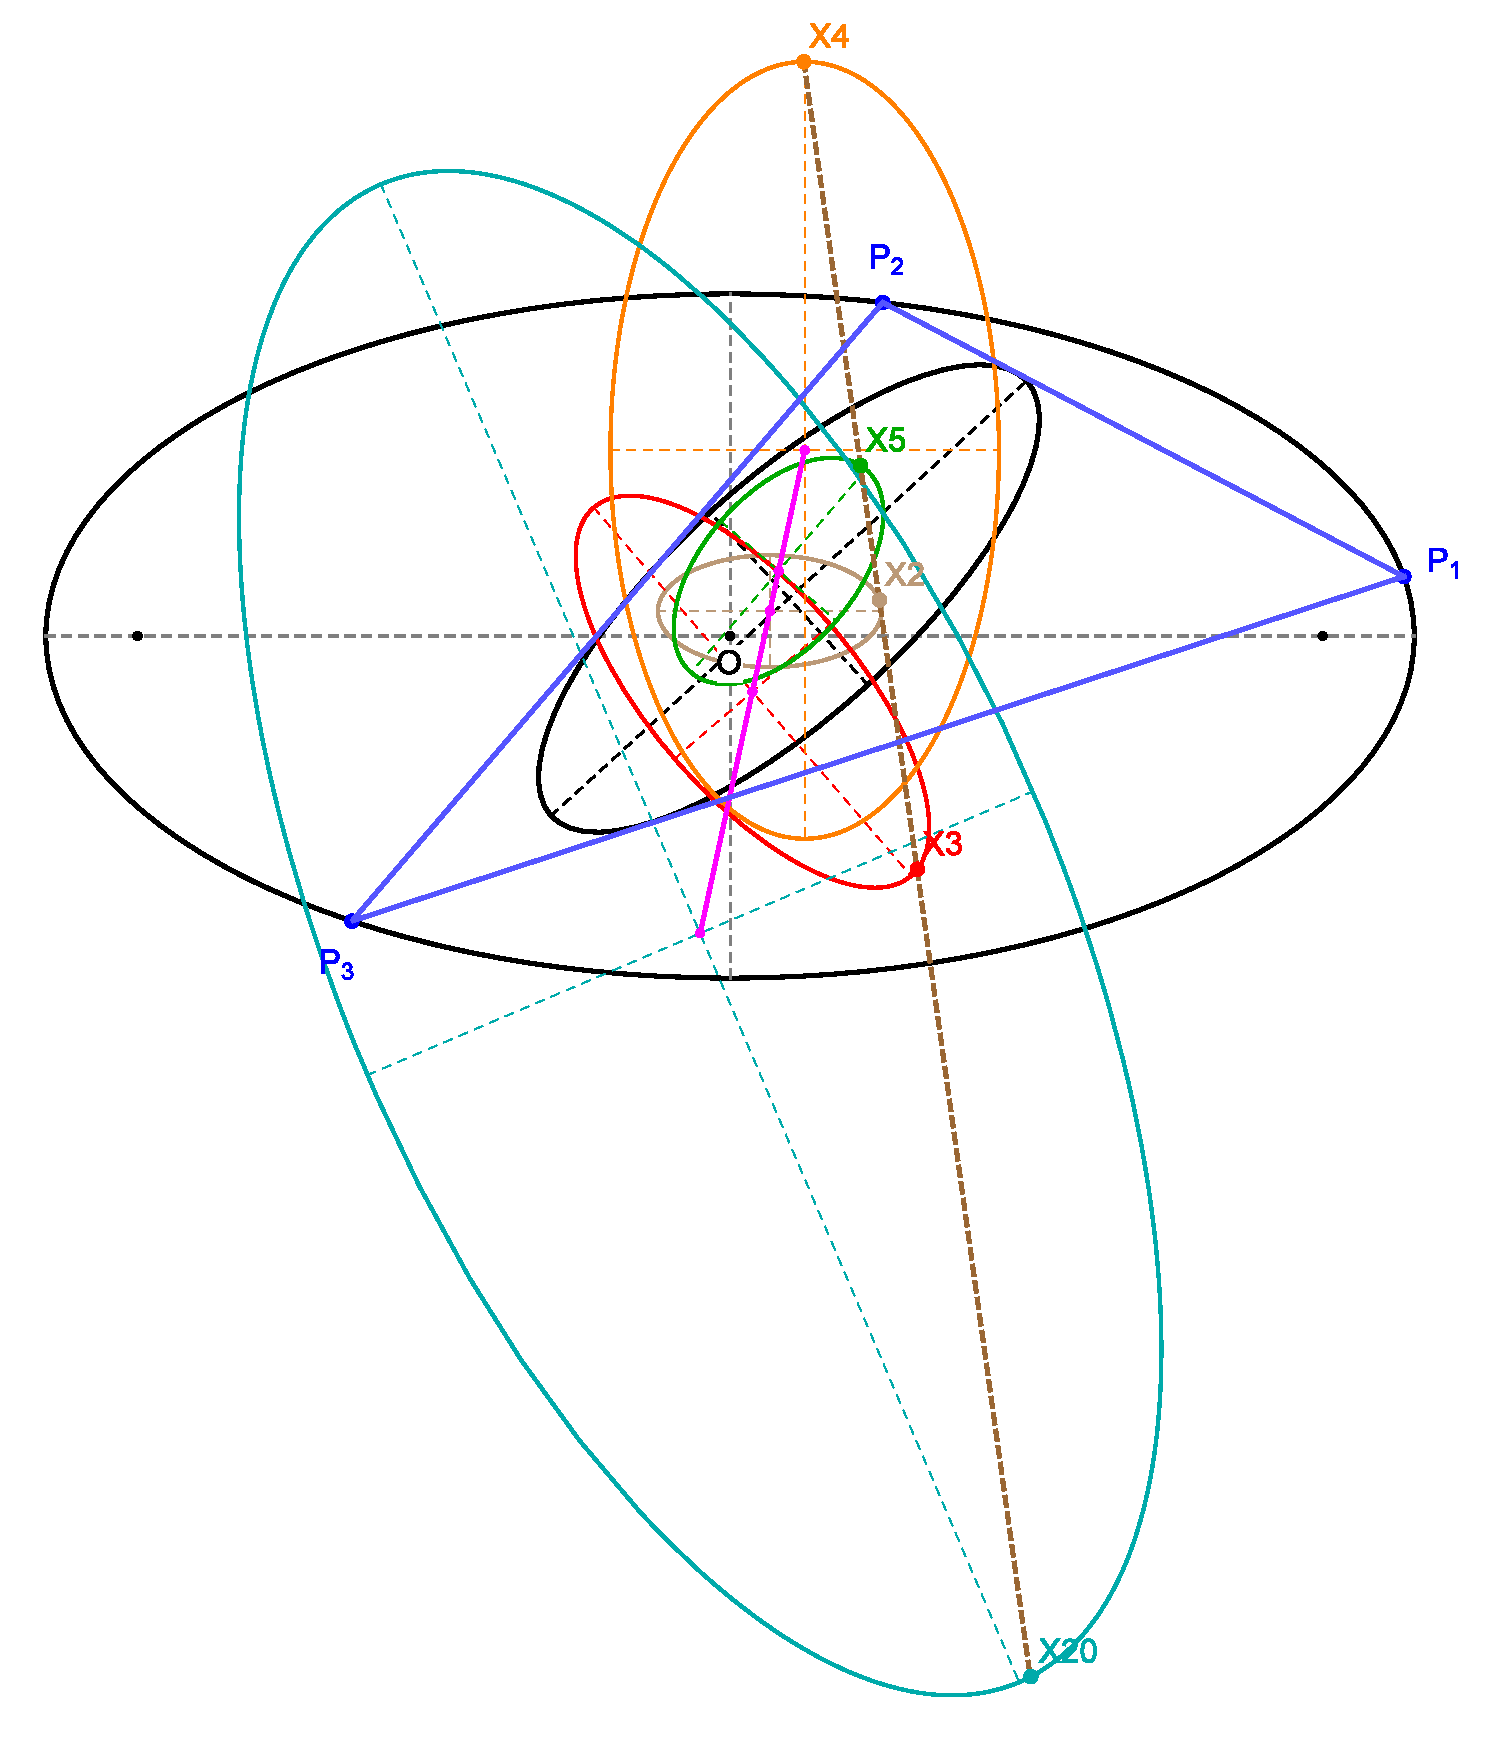
\includegraphics[width=.8\textwidth]{pics_03_010_n3_nonconcentric_conics.eps}
     \caption{A 3-periodic is shown interscribed between two non-concentric, non-aligned ellipses (black). The loci of $X_k$, $k=2,3,4,5,20$ (and many others) are elliptic. Those of $X_2$ and $X_4$ are axis-aligned with the outer ellipse. Furthermore, the centers of all elliptic loci are collinear (magenta line).}
     \label{fig:nonconcentric-xns}
 \end{figure}
 
\section{Locus of Incenter and Excenters}\label{sec:inc_excenter}

\begin{theorem}
Over the family of 3-periodics interscribed in a generic nested pair of ellipses (non-concentric, non-axis-aligned),
if $\X\ab$ is a fixed linear combination of $X_2$ and $X_3$, i.e., $\X\ab=\alpha X_2+\beta X_3$ for some fixed $\alpha,\beta\in\mathbb{C}$, then its locus is an ellipse. 
\label{thm:ellipse-locus}
\end{theorem}


\begin{theorem}
Over 3-periodics in the elliptic billiard (confocal pair) the locus of the incenter $X_1$ is an ellipse given by 
$x^2/a_1^2+y^2/b_1^2=1$, where
	\begin{equation*}\label{eq:Eint}\aligned
	a_1 =& \frac{\delta-b^2 }{a},\;\;\;
	%
	b_1  =   \frac{a^2-\delta}{b},\;\;\; \delta=\sqrt{a^4-a^2b^2+b^4}.
	%
	\endaligned
	\end{equation*}
	
	The locus of the Excenters (triangle formed by the intersection of external bisectors) is an ellipse with axes:
 
\begin{equation*}
 a_e=\frac{{b}^{2}+\delta}{a},\;\;\; 
 b_e=\frac{{a}^{2}+\delta}{b}
\end{equation*}
 
\noindent Notice it is similar to the $X_1$ locus, i.e., $a_1/b_1=b_e/a_e$.
\end{theorem}

A list of the elliptic loci of centers in the $X_{1}$ to $X_{200}$ range can be found \href{https://dan-reznik.github.io/why-so-many-ellipses/}{here}.

\section{Future Work}

\begin{conjecture}
The locus of the incenter is an ellipse if and only if the Poncelet ellipse pair is confocal.
\end{conjecture}

Let  $\mathbb{T } = \{ z\in \mathbb{C}: |z| = 1\} $ the unit circle and $\mathbb{D} = \{ z\in\mathbb{C} : |z| < 1\} $ the open unit disk
bounded by $\mathbb{T }.$

\begin{lemma}
If $u,v,w\in\mathbb{C}$ and $\lambda$ is a parameter that varies over the unit circle $\T\subset\mathbb{C}$, then the curve parametrized by
\[ F(\lambda)=u \lambda+ \frac{v}{\lambda}+w \]
is an ellipse centered at $w$, with semiaxis $|u|+|v|$ and $\big||u|-|v|\big|$, rotated with respect to the horizontal axis of $\mathbb{C}$ by an angle of $(\arg u+\arg v)/2$.
\label{lem:ell-param}
\end{lemma}
\begin{proof}

\end{proof}


Consider the Moebius map $M_{z_0}=(z_0-z)/(1-\overline{z_0} z)$ and the Blaschke product of degree 3 given by   $B=M_{z_0} M_{z_1} M_{z_2}$.
\begin{theorem}
Let $B$ be a Blaschke product of degree 3 with
zeros $0, f, g.$ For $\lambda \in \mathbb{T}$, let $z_1, z_2, z_3 $ denote the three distinct solutions to $ B(z) = \lambda$. Then the
lines joining $z_j$ and $z_k$, $(j \ne k)$ are tangent to the ellipse given by
\[|w - f| + |w - g| = |1 -   \overline{f}   g |.\]
\end{theorem}

\begin{theorem}
 Given two points $f,g\in\mathbb{D}$. Then there exists a unique conic $\mathcal{E}$ with the foci
$f,g$   which is 3-Poncelet caustic with respect to $\mathbb{T}$. Moreover, $\mathcal{E}$ is an ellipse. That ellipse is
the Blaschke ellipse with the major axis of length $|1-\overline{f}g|.$
\end{theorem}

Consider the parametrization of a triangular orbit $\{z_1,z_2,z_3\}$ as given in \cite{helman2021-power-loci}.
Let also the  affine transformation
$T(z)=pz+q\ol z$.
\begin{definition}[Blaschke's Parametrization]
\begin{align*}
    \sigma_1:=z_1+z_2+z_3=& f+g+\l\ol f \ol g =\alpha\\
    \sigma_2:=z_1 z_2+z_2 z_3+z_3 z_1=& f g+\l(\ol f+\ol g) =\beta\\
    \sigma_3:=z_1 z_2 z_3=& \l
\end{align*}
where $f,g$ are the foci of the inner ellipse and $\l\in\T$ is the varying parameter.
\label{def:bla}
\end{definition}
\begin{proposition}\label{prop:X1c}
Over Poncelet 3-periodics in the pair with an outer circle and an ellipse in generic position, the locus $X_1$ given by:
\begin{align*}
  X_1:&\;z^4 - 2(( \bar{f} + \bar{g}) \lambda +  f g) z^2 + 8   \lambda z\\
  &+ (\bar{f} - \bar{g})^2 \lambda^2 +2 (  |f|^2 g +   f |g|^2 - 2 f - 2 g) \lambda + f^2 g^2=0\\
  \;&:\;  z^4 - 2\beta  z^2+ 8\lambda z+  (\beta^2-4\alpha\lambda) =0
\end{align*}
\end{proposition}

\begin{proof} The incenter of a triangle with vertices $\{z_1,z_2,z_3\}$ is given by:
\begin{align*}
    X_1&=\frac{\sqrt{a}\;z_1+\sqrt{b}\;z_2+\sqrt{c}\;z_3}{\sqrt{a}+\sqrt{b}+\sqrt{c}}\\
    a&=|z_2-z_3|^2, \; b=|z_1-z_3|^2, \;\; c=|z_2-z_1|^2
\end{align*}
Using that $z_i\in \T$ it follows that
\[a=2-(\frac{z_3}{z_2}+\frac{z_3}{z_2}),\;\; b=2-(\frac{z_1}{z_3}+\frac{z_3}{z_1}),\;\;c=2-(\frac{z_1}{z_2}+\frac{z_2}{z_1})\]
Eliminating the square roots in  the equation $X_1-z=0$ and using the relations  $\sigma_i$ (i=1,2,3) given in Blaschke's parametrization the result follows.
\end{proof}

\begin{proposition}
\label{prop:X1g}
Over Poncelet 3-periodics in a generic nested ellipse pair, the locus of $X_1$ is given by the following sextic polynomial in $z,\lambda$:
{\small
\begin{align*}
X_1&: \;{\lambda}^{2} \left( p^2-q^2 \right) {
z}^{4}+4\,\lambda\, \left( \alpha\,\lambda\,p q^2  - q\,{
\lambda}^{2}p^{2}-\beta\,p^2\,q+p\,q^{2} \right) {z}^{3}\\
&+  ( 4\,\alpha\,{
\lambda}^{3}p^{3} q-4\,{\alpha}^{2}{\lambda}^{2}p^{2}q^2 +2\,\alpha\,\beta\,\lambda\,p^{3}
\,q-2\,\alpha\,\beta\,\lambda\,pq^{3} -2\,\beta\,{\lambda}^{2
}p^{4}+6\,\beta\,{\lambda}^{2}p^{2}q^2\\
&-6\,\alpha\,
\lambda\,p^2\,q^{2}+2\,\alpha\,\lambda\,q^{3} q+4\,{
\beta}^{2}p^2\,q^{2}  
  +6\,{\lambda}^{2}p^{3} \,q
 -6\,{
\lambda}^{2} p q^{3}  -4\,\beta\,p\,q^{3}  ) {z}^{
2}\\
&+ ( 4 q (\alpha^2\beta p^2 q^2 + 2\alpha^2 p^2  p q - \alpha^2 p q^3 + \beta^2 p^4 - 2\beta^2 p^2 q^2+ 4\beta p q^3 - p^2 q^2 - 2 q^4)\lambda \\
&- 4\alpha  p q^2 (\beta^2 p^2 - q^2) - 4 p^3 (\beta p  q - 2 p^2 - q^2)\lambda^3 - 16\alpha\lambda^2 p^4   q ) z\\
   & -\lambda^2 (4 \alpha \lambda - \beta^2) p^6 + 4 p^5 q \lambda^4 + 2 \lambda (4 \alpha^2 \lambda - \alpha \beta^2 - 3 \beta \lambda) p^5 q   - \lambda^2 (8 \alpha \lambda - 3 \beta^2) p^4 q^2 \\
   &+ (\alpha^2 \beta^2 -4 \alpha^3 \lambda  + 4 \alpha \beta \lambda + 5 \lambda^2) p^4 q^2 + 2 \lambda (2 \alpha^2 \lambda - \alpha \beta^2 + \beta \lambda) p^3 q^3 \\
   &+ (2 \alpha^2 \beta - 2 \alpha \lambda - 4 \beta^2) p^3 q^3 - (\alpha^2 \beta^2 + 4 \alpha \beta \lambda - 4 \beta^3 + 5 \lambda^2) p^2 q^4 + ( 8 \beta-3 \alpha^2 ) p^2 q^4 \\
   &+ (2 \alpha^2 \beta + 6 \alpha \lambda - 8 \beta^2) p q^5 - 4 q^5 p + ( 4 \beta-\alpha^2 ) q^6=0
\end{align*}
}
\end{proposition}

\begin{proof} Let $p,q\in \mathbb{R}$. Consider the affine transformation
$T(z)=pz+q\ol z$ and set $w_i=T(z_i)$. The proof is similar to that given in \cref{prop:X1c}.  
\end{proof}

\begin{proposition} In the confocal pair the locus $X_1$ is defined by:
\[2\,ab{\lambda}^{2}{z}^{2}+2\,\lambda\, \left( {a}^{3}{\lambda}^{2}-{b}
^{3}{\lambda}^{2}-{a}^{3}-{b}^{3} \right) z+{c}^{2} \left( {c}^{2}{
\lambda}^{4}-2\,ab{\lambda}^{2}-{c}^{2} \right)=0 \]
\label{prop:X1q2} 
\end{proposition}

\begin{proof}
We have that
\[f={\frac {1}{c}\sqrt {-{a}^{2}-{b}^{2}+2\,\delta}}, \;\; g= -{\frac {1}{c}\sqrt {-{a}^{2}-{b}^{2}+2\,\delta}}\]

\end{proof}

\begin{corollary}
The locus $X_1$ is the ellipse with semiaxes given by $a_1=(a^2-\delta)/b$ and $b_1=(\delta-b^2)/a.$

%\[z= {\frac { \left( a-b \right)  \left(\delta -{a}^{2}-ab-{b}^{2}
 %\right) \lambda}{2\,ab}}-{\frac { \left( a+b %\right)  \left(  \delta-{a}^{2}
%+ab-{b}^{2} \right) }{2\,ab\lambda}}\]
 
\end{corollary}

\begin{proof}
The quartic polynomial is factorizable as $p_1p_2$, where
\begin{align*}
    p_1&=z-\left({\frac { \left( a-b \right)  \left( -{a}^{2}-a b-{b}^{2}+\delta
 \right) \lambda}{2\,a b}}-{\frac { \left( a+b \right)  \left( -{a}^{2}
+a b-{b}^{2}+\delta \right) }{2\,a b\lambda}}\right)
\\
    p_2&=2 a b \lambda^2 z^3 - ((a - b) (a^2 + 3 a b + b^2 + \delta) \lambda^3 - (a + b) (a^2 - 3 a b + b^2 + \delta) \lambda) z^2\\
    &+ 6 a b  (a^2 - b^2) \lambda^2 z + (a + b)^3 (a^2 - a b + b^2 + \delta) \lambda^3 - (a - b)^3 (a^2 + a b + b^2 + \delta) \lambda
\end{align*}
Follows directly from  \cref{lem:ell-param} and  \cref{prop:X1q2}.
\end{proof}

\cite{schwartz2016-com}

\begin{conjecture}
Over 3-periodics interscribed between two ellipses in general position, the locus of a triangle center $X_k$ is an ellipse if and only if $X_k$ is a fixed linear combination of $X_3$ and $X_4$.
\end{conjecture}